\lstinputlisting[language=bash,basicstyle=\small]{python_codes/fieldstone_80/keywords}

\begin{center}
Code at \url{https://github.com/cedrict/fieldstone/tree/master/python_codes/fieldstone_80}
\end{center}

\par\noindent\rule{\textwidth}{0.4pt}
%%%%%%%%%%%%%%%%%%%%%%%%%%%%%%%%%%%%%%%%%%%%%%%%%%%%%%%%%%%%%%%%%%%%%%%%%%%%%%%%%%%%%%%%%%%%%%

We here consider the enriched $Q_1\times P_0$ element introduced first by Fortin (1981) \cite{fort81}.
The shape functions in 2D and 3D are in derived in Section~\ref{ss:Q1pP02D} and Section~\ref{ss:Q1pP03D} respectively.


Per element:
\[
\vec{V} = (u_1,v_1,u_2,v_2,u_3,v_3,u_4,v_4,u_5,v_5,u_6,v_6)
\]

Here is a 4x3 element mesh. Bubble $u$ dofs are represented in blue and bubble $v$ dofs are shown in green.


\begin{center}
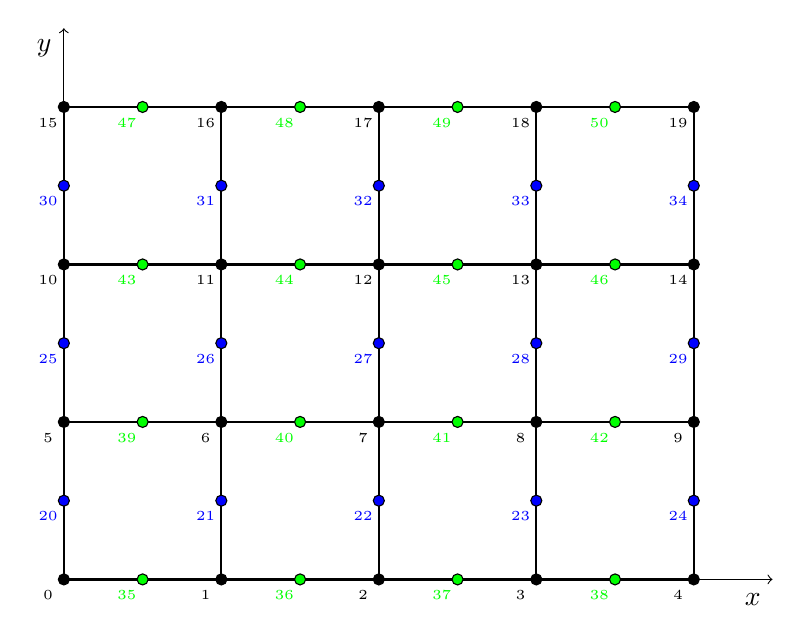
\begin{tikzpicture}
%\draw[fill=gray!23,gray!23](0,0) rectangle (10,8);
%\draw[step=0.5cm,gray,very thin] (0,0) grid (10,8); %background grid

\draw[thick] (1,1) -- (9,1) ;
\draw[thick] (1,3) -- (9,3) ;
\draw[thick] (1,5) -- (9,5) ;
\draw[thick] (1,7) -- (9,7) ;

\draw[thick] (1,1) -- (1,7) ;
\draw[thick] (3,1) -- (3,7) ;
\draw[thick] (5,1) -- (5,7) ;
\draw[thick] (7,1) -- (7,7) ;
\draw[thick] (9,1) -- (9,7) ;

\draw[black,fill=black] (1,1)   circle (2pt);
\draw[black,fill=black] (3,1)   circle (2pt);
\draw[black,fill=black] (5,1)   circle (2pt);
\draw[black,fill=black] (7,1)   circle (2pt);
\draw[black,fill=black] (9,1)   circle (2pt);

\draw[black,fill=black] (1,3)   circle (2pt);
\draw[black,fill=black] (3,3)   circle (2pt);
\draw[black,fill=black] (5,3)   circle (2pt);
\draw[black,fill=black] (7,3)   circle (2pt);
\draw[black,fill=black] (9,3)   circle (2pt);

\draw[black,fill=black] (1,5)   circle (2pt);
\draw[black,fill=black] (3,5)   circle (2pt);
\draw[black,fill=black] (5,5)   circle (2pt);
\draw[black,fill=black] (7,5)   circle (2pt);
\draw[black,fill=black] (9,5)   circle (2pt);

\draw[black,fill=black] (1,7)   circle (2pt);
\draw[black,fill=black] (3,7)   circle (2pt);
\draw[black,fill=black] (5,7)   circle (2pt);
\draw[black,fill=black] (7,7)   circle (2pt);
\draw[black,fill=black] (9,7)   circle (2pt);

\draw[black,fill=blue] (1,2) circle (2pt); 
\draw[black,fill=blue] (3,2) circle (2pt); 
\draw[black,fill=blue] (5,2) circle (2pt); 
\draw[black,fill=blue] (7,2) circle (2pt); 
\draw[black,fill=blue] (9,2) circle (2pt); 

\draw[black,fill=blue] (1,4) circle (2pt); 
\draw[black,fill=blue] (3,4) circle (2pt); 
\draw[black,fill=blue] (5,4) circle (2pt); 
\draw[black,fill=blue] (7,4) circle (2pt); 
\draw[black,fill=blue] (9,4) circle (2pt); 

\draw[black,fill=blue] (1,6) circle (2pt); 
\draw[black,fill=blue] (3,6) circle (2pt); 
\draw[black,fill=blue] (5,6) circle (2pt); 
\draw[black,fill=blue] (7,6) circle (2pt); 
\draw[black,fill=blue] (9,6) circle (2pt); 

\draw[black,fill=green] (2,1) circle (2pt); 
\draw[black,fill=green] (4,1) circle (2pt); 
\draw[black,fill=green] (6,1) circle (2pt); 
\draw[black,fill=green] (8,1) circle (2pt); 

\draw[black,fill=green] (2,3) circle (2pt); 
\draw[black,fill=green] (4,3) circle (2pt); 
\draw[black,fill=green] (6,3) circle (2pt); 
\draw[black,fill=green] (8,3) circle (2pt); 

\draw[black,fill=green] (2,5) circle (2pt); 
\draw[black,fill=green] (4,5) circle (2pt); 
\draw[black,fill=green] (6,5) circle (2pt); 
\draw[black,fill=green] (8,5) circle (2pt); 

\draw[black,fill=green] (2,7) circle (2pt); 
\draw[black,fill=green] (4,7) circle (2pt); 
\draw[black,fill=green] (6,7) circle (2pt); 
\draw[black,fill=green] (8,7) circle (2pt); 

\draw[thin,->] (9,1) -- (10,1); %x
\draw[thin,->] (1,7) -- (1,8); %y
\node[] at (9.75,0.75) {$x$};
\node[] at (0.75,7.75) {$y$};

\node[] at (0.8,0.8) {\tiny 0};
\node[] at (2.8,0.8) {\tiny 1};
\node[] at (4.8,0.8) {\tiny 2};
\node[] at (6.8,0.8) {\tiny 3};
\node[] at (8.8,0.8) {\tiny 4};
\node[] at (0.8,2.8) {\tiny 5};
\node[] at (2.8,2.8) {\tiny 6};
\node[] at (4.8,2.8) {\tiny 7};
\node[] at (6.8,2.8) {\tiny 8};
\node[] at (8.8,2.8) {\tiny 9};
\node[] at (0.8,4.8) {\tiny 10};
\node[] at (2.8,4.8) {\tiny 11};
\node[] at (4.8,4.8) {\tiny 12};
\node[] at (6.8,4.8) {\tiny 13};
\node[] at (8.8,4.8) {\tiny 14};
\node[] at (0.8,6.8) {\tiny 15};
\node[] at (2.8,6.8) {\tiny 16};
\node[] at (4.8,6.8) {\tiny 17};
\node[] at (6.8,6.8) {\tiny 18};
\node[] at (8.8,6.8) {\tiny 19};

\node[] at (0.8,1.8) {\tiny \color{blue} 20};
\node[] at (2.8,1.8) {\tiny \color{blue} 21};
\node[] at (4.8,1.8) {\tiny \color{blue} 22};
\node[] at (6.8,1.8) {\tiny \color{blue} 23};
\node[] at (8.8,1.8) {\tiny \color{blue} 24};

\node[] at (0.8,3.8) {\tiny \color{blue} 25};
\node[] at (2.8,3.8) {\tiny \color{blue} 26};
\node[] at (4.8,3.8) {\tiny \color{blue} 27};
\node[] at (6.8,3.8) {\tiny \color{blue} 28};
\node[] at (8.8,3.8) {\tiny \color{blue} 29};

\node[] at (0.8,5.8) {\tiny \color{blue} 30};
\node[] at (2.8,5.8) {\tiny \color{blue} 31};
\node[] at (4.8,5.8) {\tiny \color{blue} 32};
\node[] at (6.8,5.8) {\tiny \color{blue} 33};
\node[] at (8.8,5.8) {\tiny \color{blue} 34};

\node[] at (1.8,0.8) {\tiny \color{green} 35};
\node[] at (3.8,0.8) {\tiny \color{green} 36};
\node[] at (5.8,0.8) {\tiny \color{green} 37};
\node[] at (7.8,0.8) {\tiny \color{green} 38};

\node[] at (1.8,2.8) {\tiny \color{green} 39};
\node[] at (3.8,2.8) {\tiny \color{green} 40};
\node[] at (5.8,2.8) {\tiny \color{green} 41};
\node[] at (7.8,2.8) {\tiny \color{green} 42};

\node[] at (1.8,4.8) {\tiny \color{green} 43};
\node[] at (3.8,4.8) {\tiny \color{green} 44};
\node[] at (5.8,4.8) {\tiny \color{green} 45};
\node[] at (7.8,4.8) {\tiny \color{green} 46};

\node[] at (1.8,6.8) {\tiny \color{green} 47};
\node[] at (3.8,6.8) {\tiny \color{green} 48};
\node[] at (5.8,6.8) {\tiny \color{green} 49};
\node[] at (7.8,6.8) {\tiny \color{green} 50};

\end{tikzpicture}\\
\end{center}

For this mesh we have 

\begin{lstlisting}
nel=nelx*nely (=12) 
NP=nel (=12)
NV=nnx*nny+nnx*nely+nny*nelx (=20+16+15=51)
\end{lstlisting}

The total number of velocity dofs is 
\begin{lstlisting}
NfemV=ndofV*nnx*nny + nnx*nely + nny*nelx (=71)
\end{lstlisting}
while the total number of pressure dofs remains
\begin{lstlisting}
NfemP=NP*ndofP (=nel) 
\end{lstlisting}


There are two connectivity arrays {\tt iconu} and {\tt iconv}, both of size $mV\times nel$, where 
$mV=6$ is the number of nodes linked to an element. For each element, and depending on whether we are considering 
the polynomial approximation $u^h(x,y)$ or $v^h(x,y)$ in the element, there are the standard 4 $Q_1$ nodes and 2 additional 
dofs, so $mV=6$.
\begin{itemize}
\item content of {\tt iconu}
\begin{verbatim}
elt
0 | [ 0  1  6  5 20 21]
1 | [ 1  2  7  6 21 22]
2 | [ 2  3  8  7 22 23]
3 | [ 3  4  9  8 23 24]
4 | [ 5  6 11 10 25 26]
5 | [ 6  7 12 11 26 27]
6 | [ 7  8 13 12 27 28]
7 | [ 8  9 14 13 28 29]
8 | [10 11 16 15 30 31]
9 | [11 12 17 16 31 32]
10 | [12 13 18 17 32 33]
11 | [13 14 19 18 33 34]
\end{verbatim}
\item content of {\tt iconv}
\begin{verbatim}
elt
 0 | [ 0  1  6  5 35 39]
 1 | [ 1  2  7  6 36 40]
 2 | [ 2  3  8  7 37 41]
 3 | [ 3  4  9  8 38 42]
 4 | [ 5  6 11 10 39 43]
 5 | [ 6  7 12 11 40 44]
 6 | [ 7  8 13 12 41 45]
 7 | [ 8  9 14 13 42 46]
 8 | [10 11 16 15 43 47]
 9 | [11 12 17 16 44 48]
10 | [12 13 18 17 45 49]
11 | [13 14 19 18 46 50]
\end{verbatim}
\end{itemize}

The pressure field is normalised by imposing $\int_\Omega p dV=0 $ so that there is no nullspace.

%---------------------------------------------------------------
\subsection*{Donea \& Huerta manufactured solution benchmark}

The Donea \& huerta benchmark of Section~\ref{mms1} is implemented. It requires 
no-slip boundary conditions on all sides. This means that $u=0$ must be 
prescribed on the lateral boundaries, while $v=0$ is prescribed at the top and bottom, 
i.e. boundary conditions are imposed on the bubble nodes too.

\begin{center}
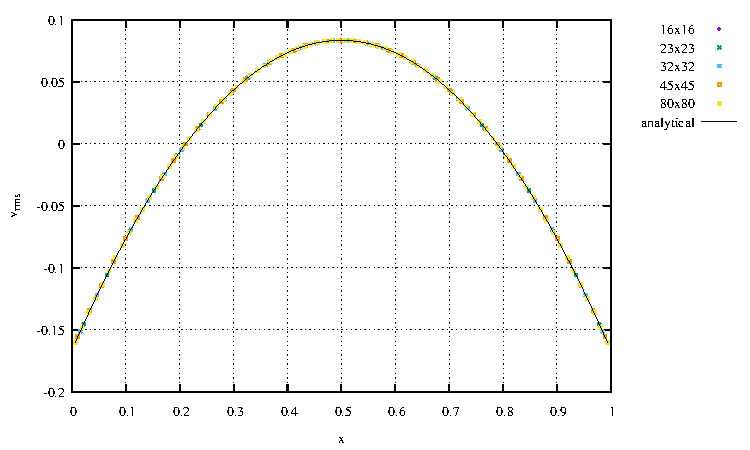
\includegraphics[width=7cm]{python_codes/fieldstone_80/results/dh/pressure}
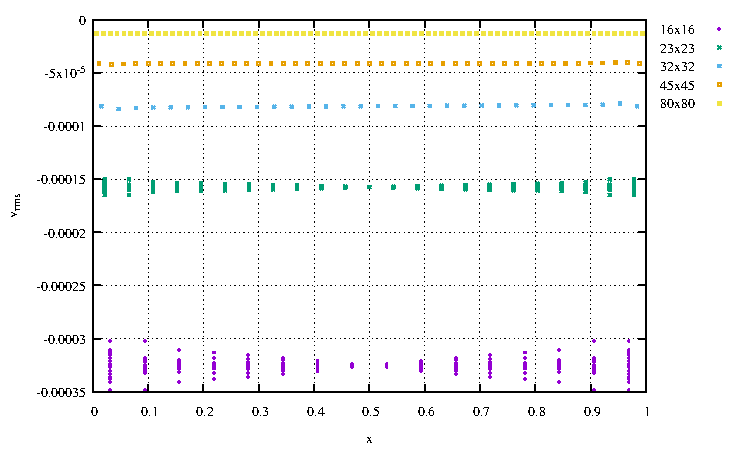
\includegraphics[width=7cm]{python_codes/fieldstone_80/results/dh/pressure_error}\\
{\captionfont  opla}
\end{center}


Looking at the velocity and pressure error convergence, we see that the number of quadrature
points does not matter much, but surprisingly the lowest number of quad points seems to yield slightly
better results...
\begin{center}
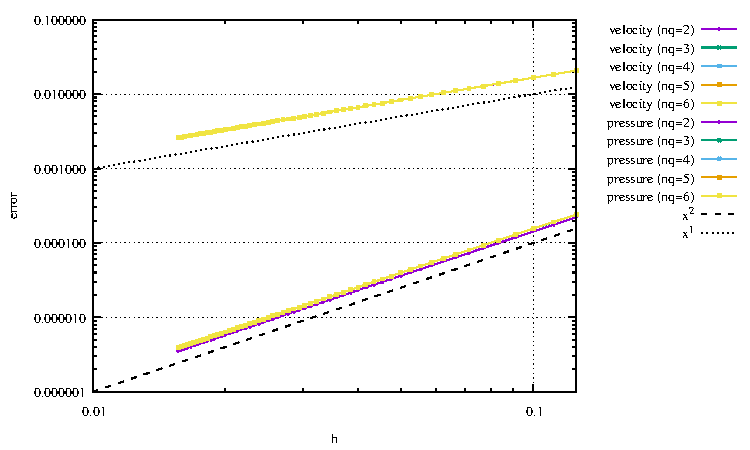
\includegraphics[width=9cm]{python_codes/fieldstone_80/results/dh/errors}\\
{\captionfont Velocity and pressure error convergence as a function of resolution for 
different quadrature rules.}
\end{center}

\begin{center}
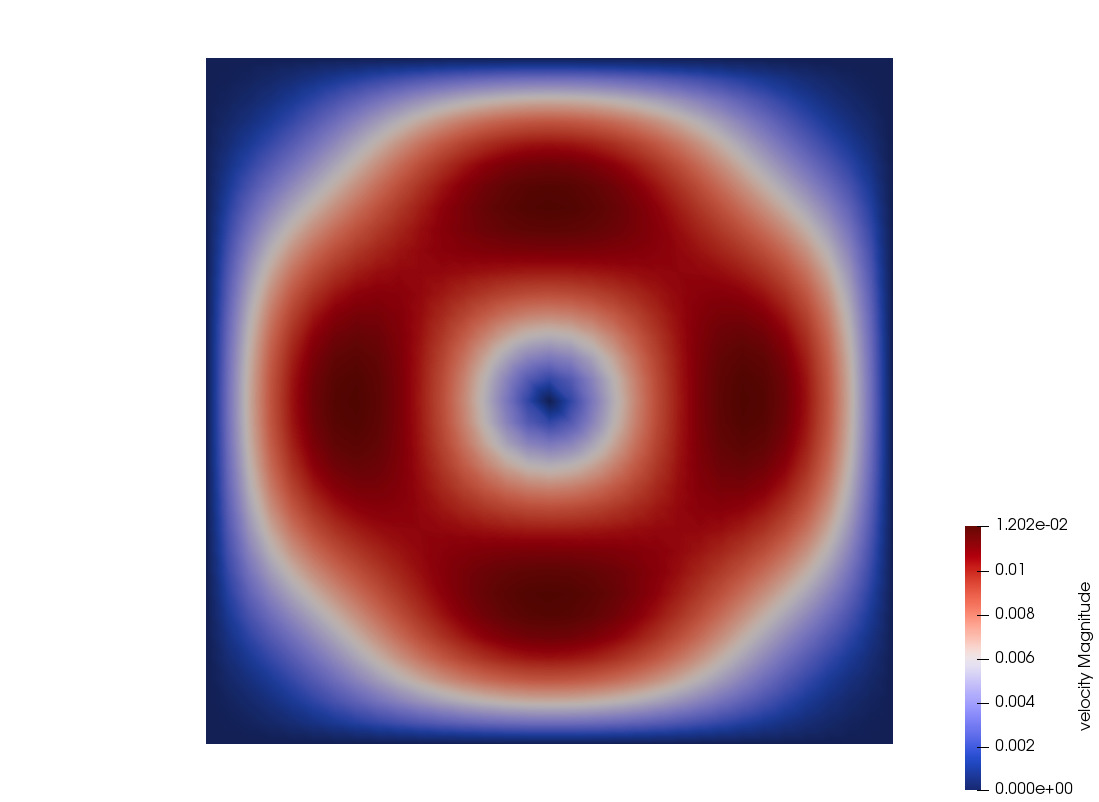
\includegraphics[width=7cm]{python_codes/fieldstone_80/results/dh/vel}
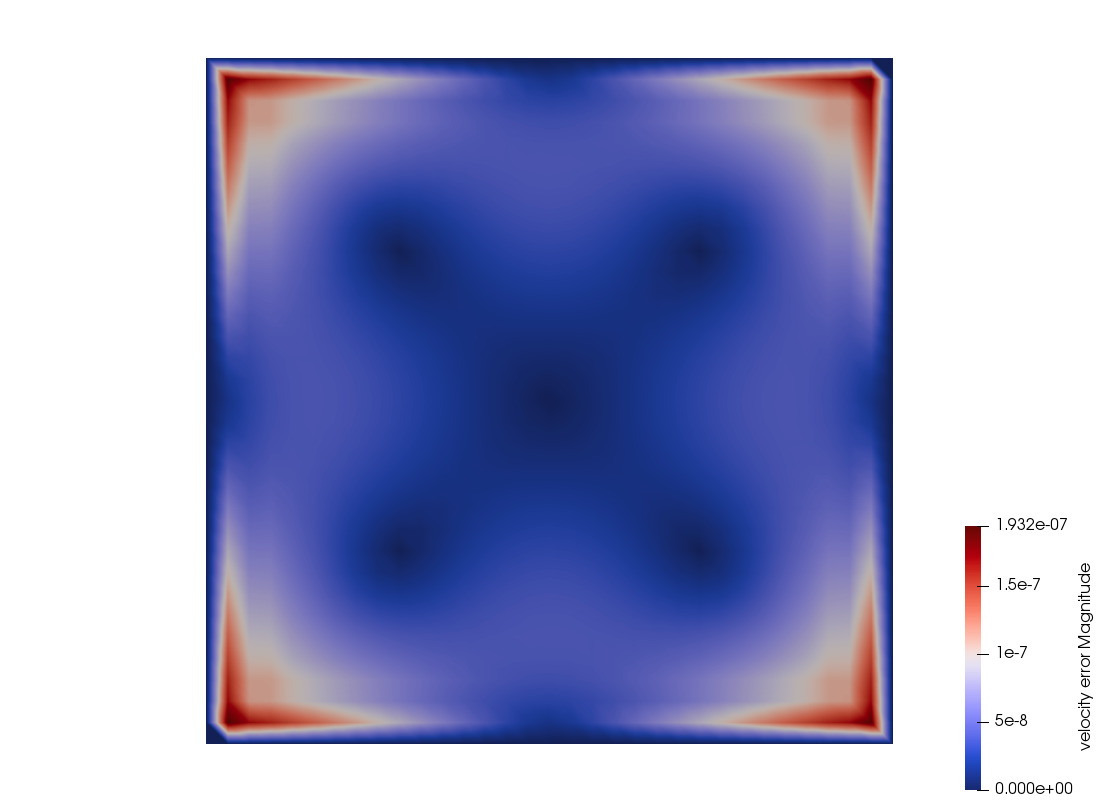
\includegraphics[width=7cm]{python_codes/fieldstone_80/results/dh/vel_error}\\
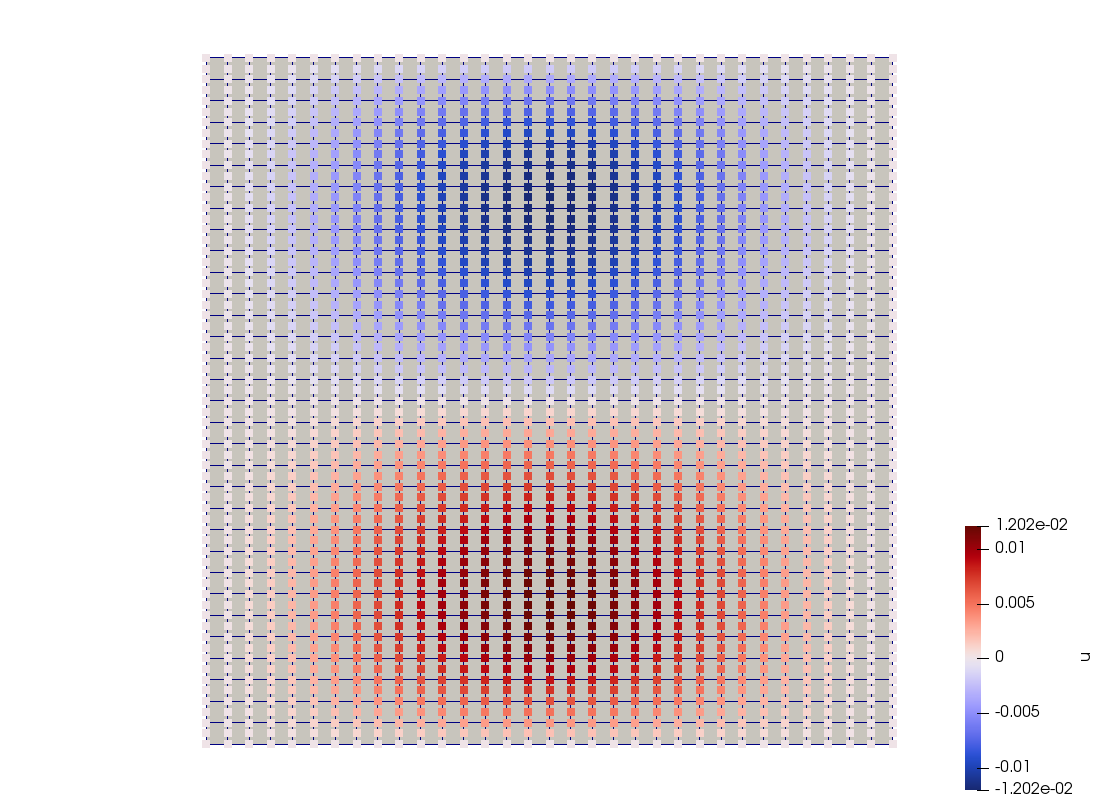
\includegraphics[width=7cm]{python_codes/fieldstone_80/results/dh/u_dofs}
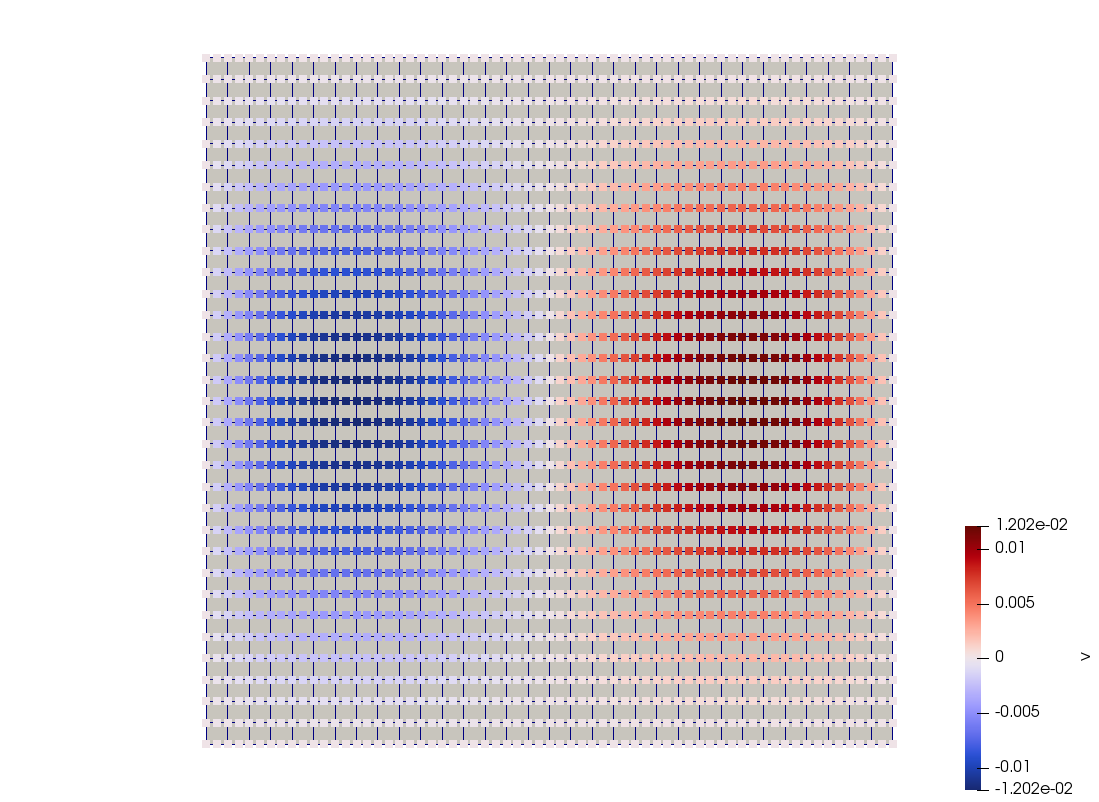
\includegraphics[width=7cm]{python_codes/fieldstone_80/results/dh/v_dofs}\\
{\captionfont Top row: velocity and velocity error. Bottom row: $u$ and 
$v$ plotted on their respective meshes.}
\end{center}

%---------------------------------------------------------------
\subsection*{The aquarium}

No-slip boundary conditions are prescribed on all sides. Density and viscosity are 1.
Gravity is $\vec{g}=-\vec{e}_y$. 

We recover a linear pressure profile as expected, that is very accurate:

\begin{center}
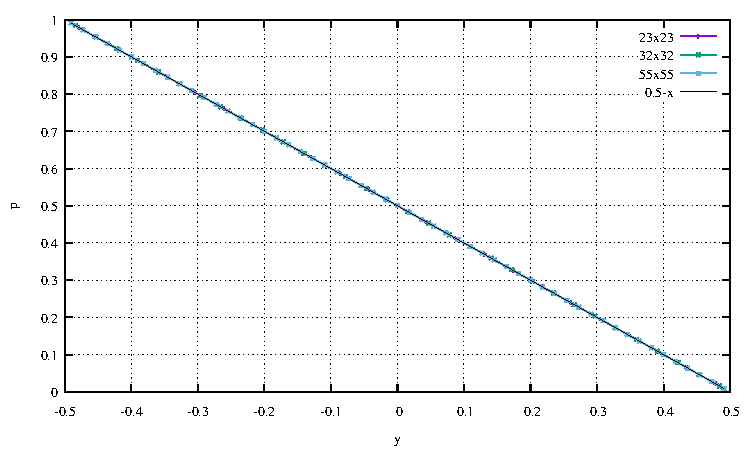
\includegraphics[width=7.5cm]{python_codes/fieldstone_80/results/aquarium/p}
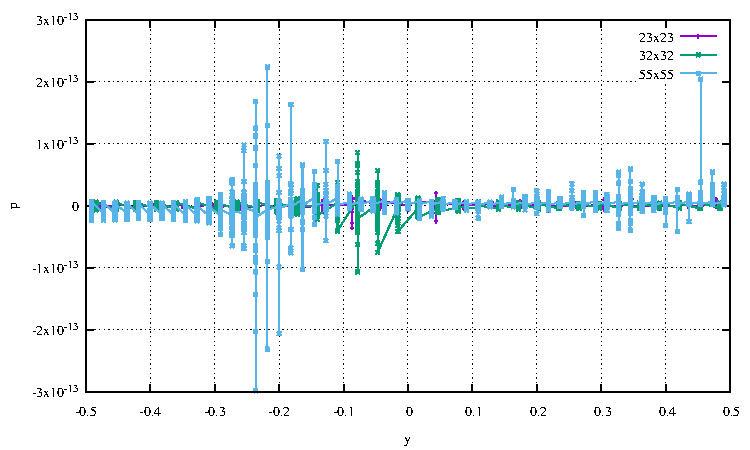
\includegraphics[width=7.5cm]{python_codes/fieldstone_80/results/aquarium/p_error}\\
{\captionfont Left: pressure profile; Right: pressure profile error}
\end{center}

We can also record the root mean square velocity as a function of the resolution $h$
and we find that the velocity is (as expected) zero (down to machine precision):
\begin{center}
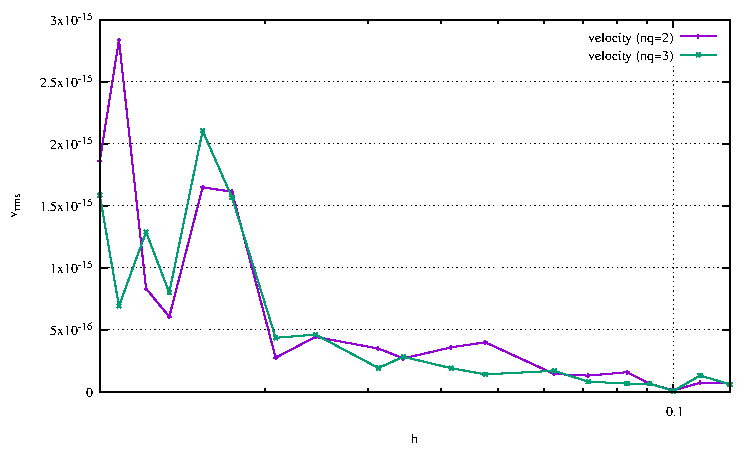
\includegraphics[width=9cm]{python_codes/fieldstone_80/results/aquarium/vrms}
\end{center}


%---------------------------------------------------------------
\subsection*{The lid driven cavity}

This is the non leaky lid driven cavity, i.e. the velocity at the top left and right corner 
is set to zero. No slip are imposed on all three other boundaries. 
The pressure field does not showcase any checkerboard mode. 

\begin{center}
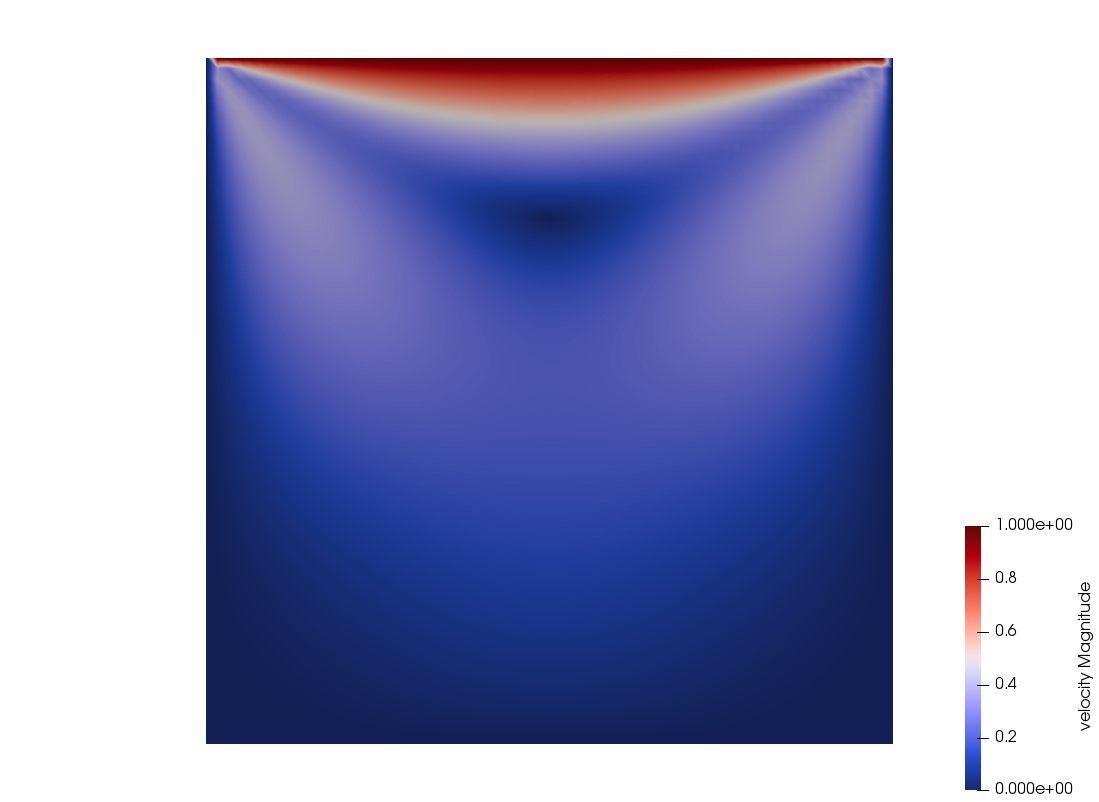
\includegraphics[width=7.5cm]{python_codes/fieldstone_80/results/ldc/vel}
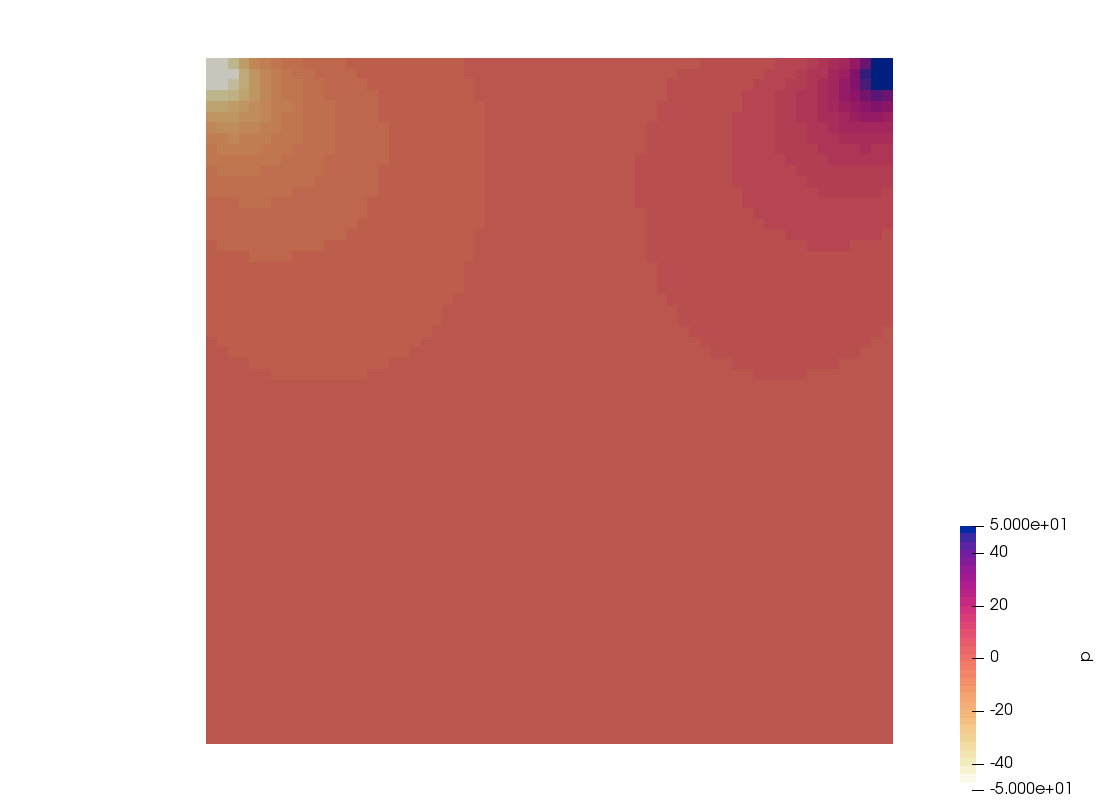
\includegraphics[width=7.5cm]{python_codes/fieldstone_80/results/ldc/p}
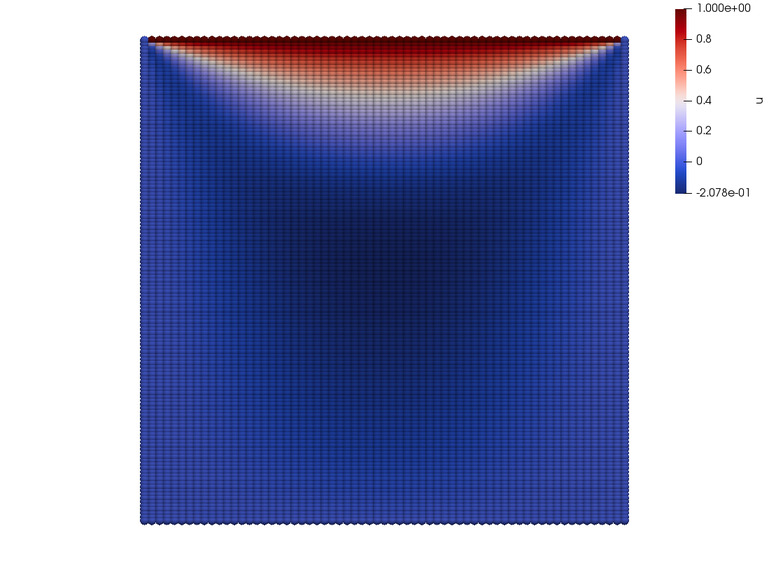
\includegraphics[width=7.5cm]{python_codes/fieldstone_80/results/ldc/u_dofs}
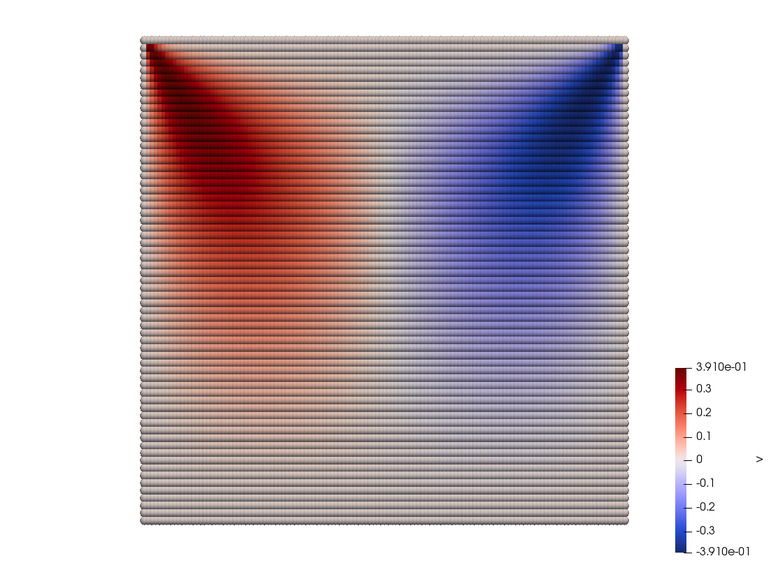
\includegraphics[width=7.5cm]{python_codes/fieldstone_80/results/ldc/v_dofs}\\
{\captionfont 64x64}
\end{center}

\begin{center}
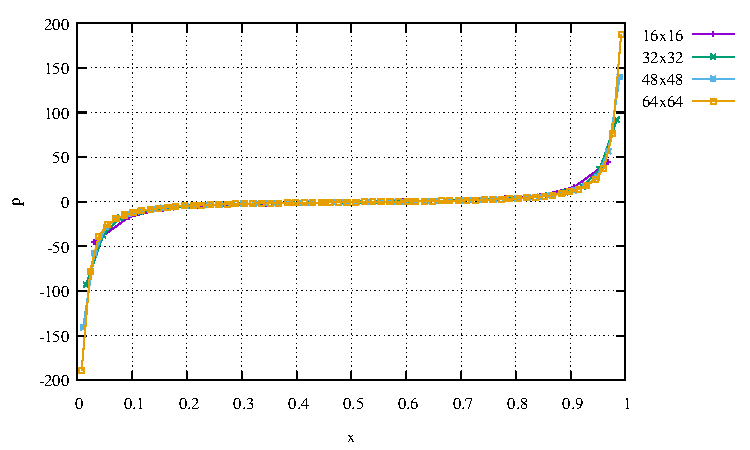
\includegraphics[width=7.5cm]{python_codes/fieldstone_80/results/ldc/p_top}
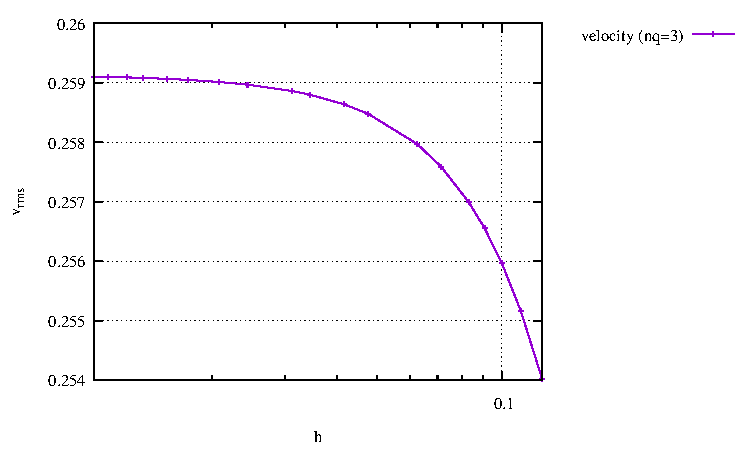
\includegraphics[width=7.5cm]{python_codes/fieldstone_80/results/ldc/vrms}
\end{center}


%---------------------------------------------------------------
\subsection*{Manufactured solution}

\begin{center}
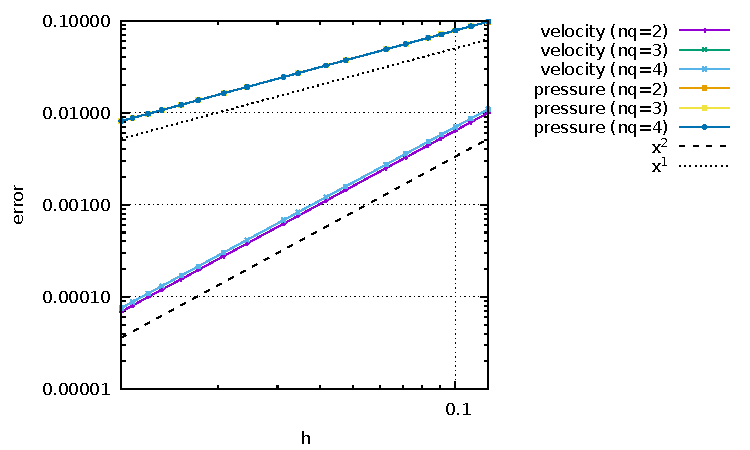
\includegraphics[width=7.5cm]{python_codes/fieldstone_80/results/lamich/errors}
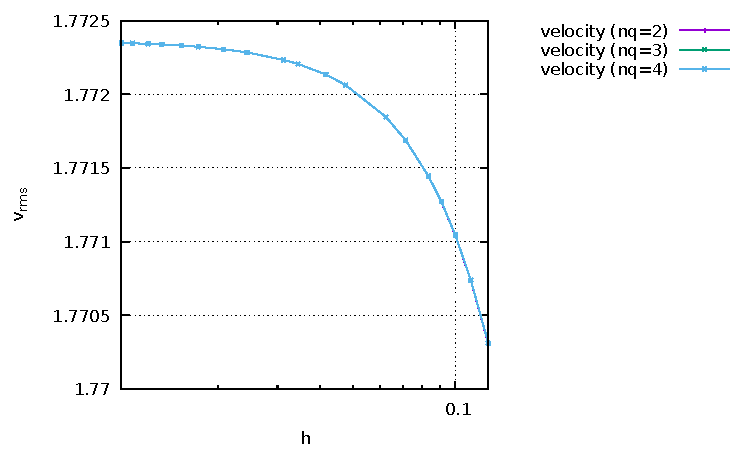
\includegraphics[width=7.5cm]{python_codes/fieldstone_80/results/lamich/vrms}\\
{\captionfont Left: Velocity and pressure error convergence; Right: root mean square velocity
as a function of mesh size.}
\end{center}


%---------------------------------------------------------------
\subsection*{Stokes sphere}

Sphere is placed in the middle with radius 0.123, free slip boundary conditions on all sides. 
Viscosity is constant in the domain. 

\begin{center}
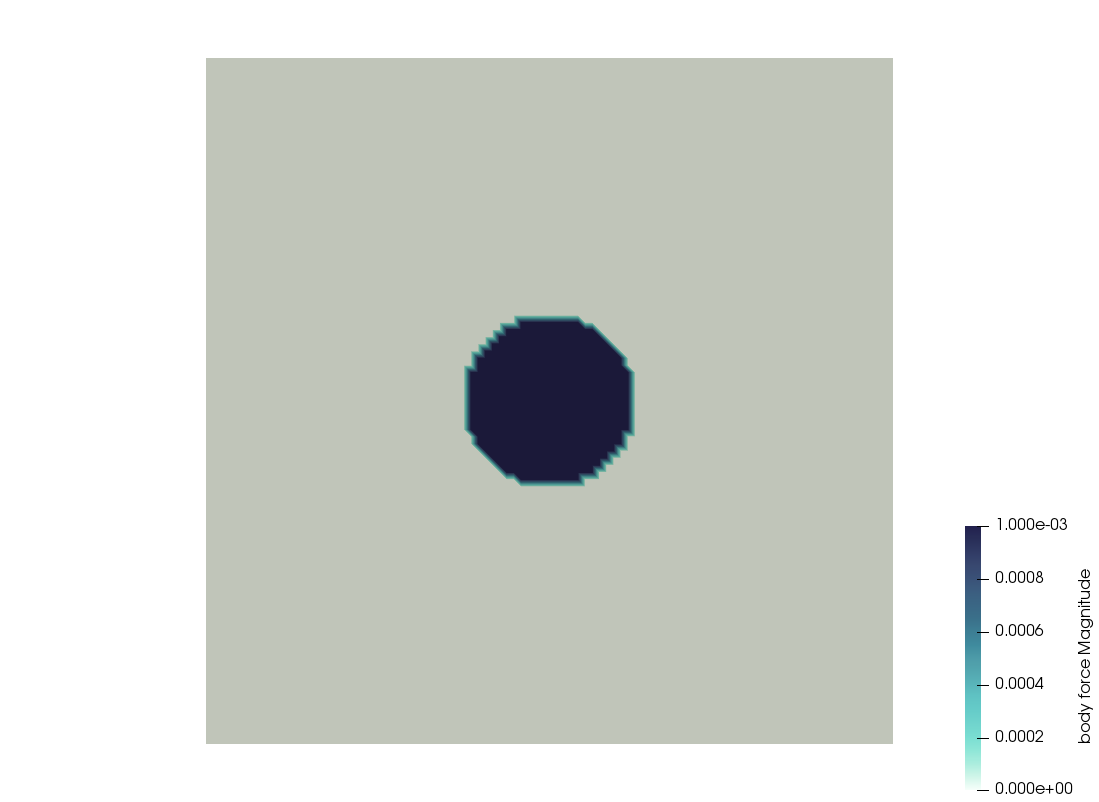
\includegraphics[width=5.6cm]{python_codes/fieldstone_80/results/sphere/rho_g}
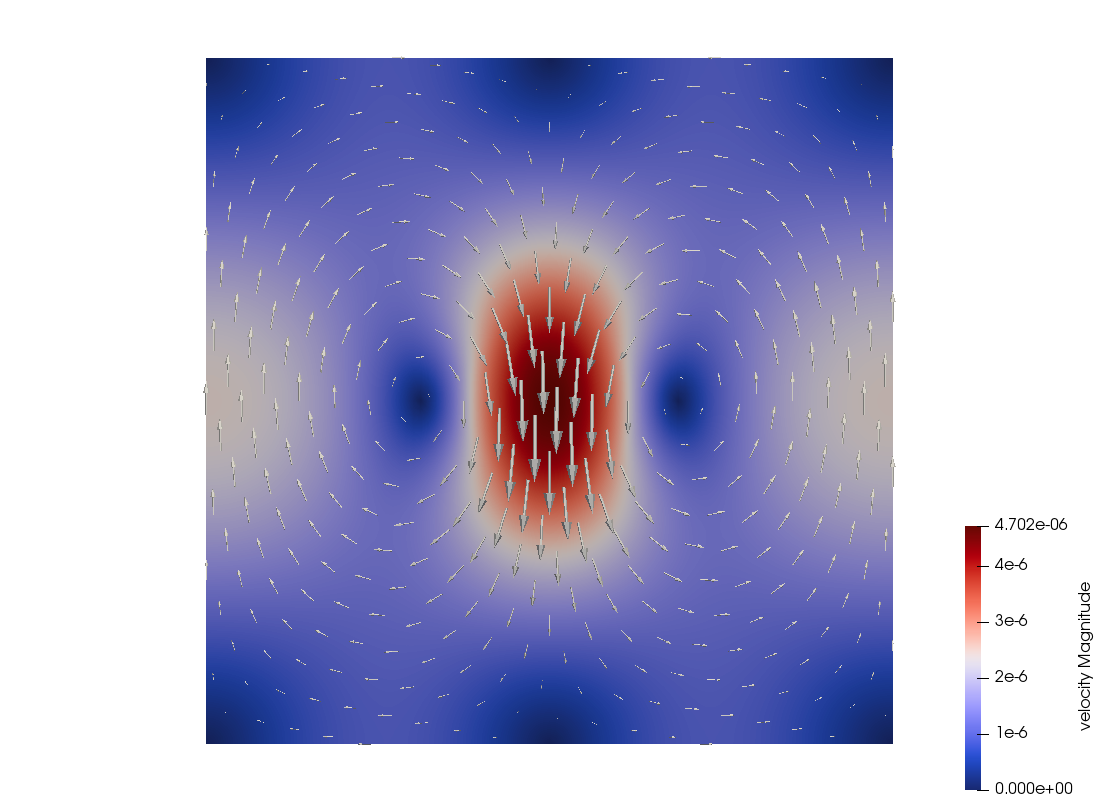
\includegraphics[width=5.6cm]{python_codes/fieldstone_80/results/sphere/vel}
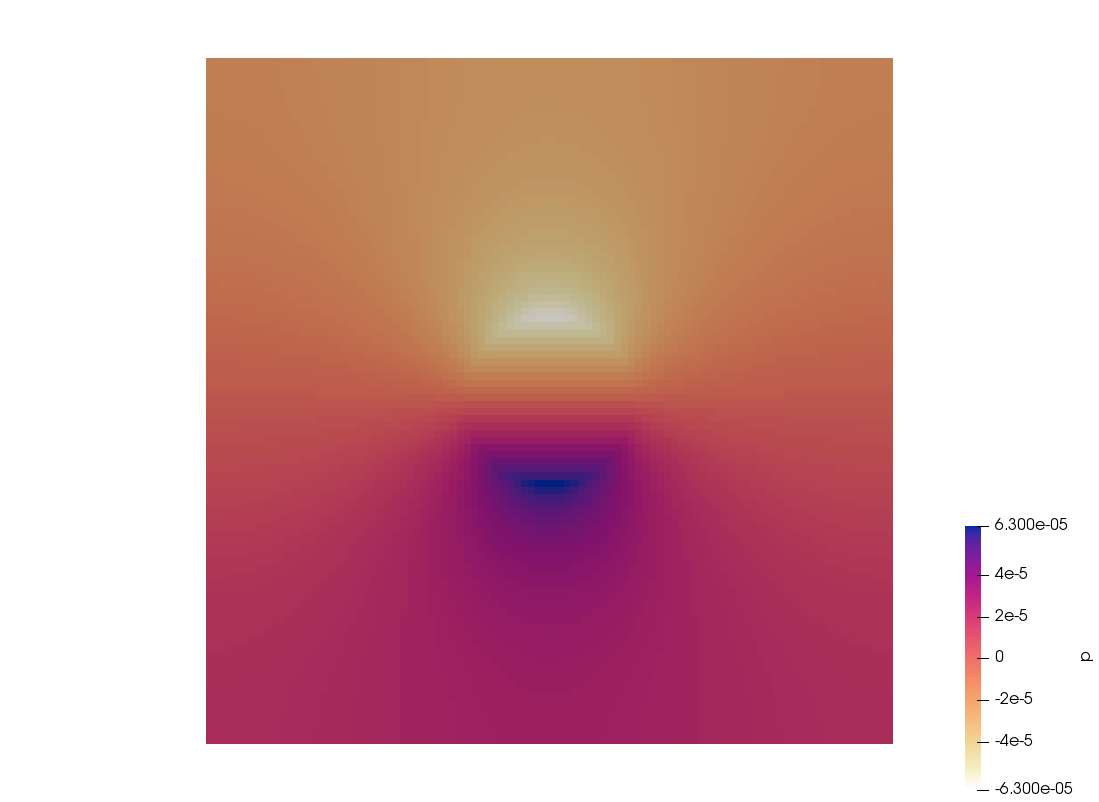
\includegraphics[width=5.6cm]{python_codes/fieldstone_80/results/sphere/p}\\
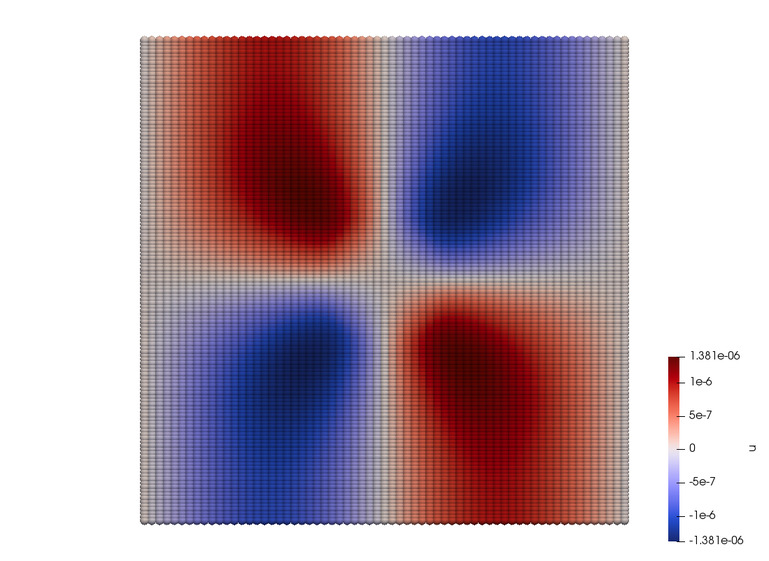
\includegraphics[width=5.6cm]{python_codes/fieldstone_80/results/sphere/u_dofs}
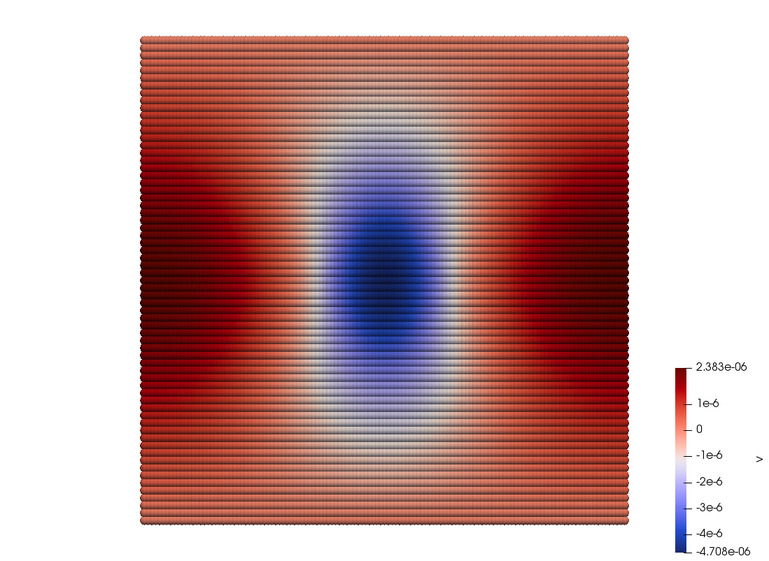
\includegraphics[width=5.6cm]{python_codes/fieldstone_80/results/sphere/v_dofs}\\
{\captionfont velocity and pressure fields for $\delta \rho=0.001$. 96x96 elements.}
\end{center}

\begin{center}
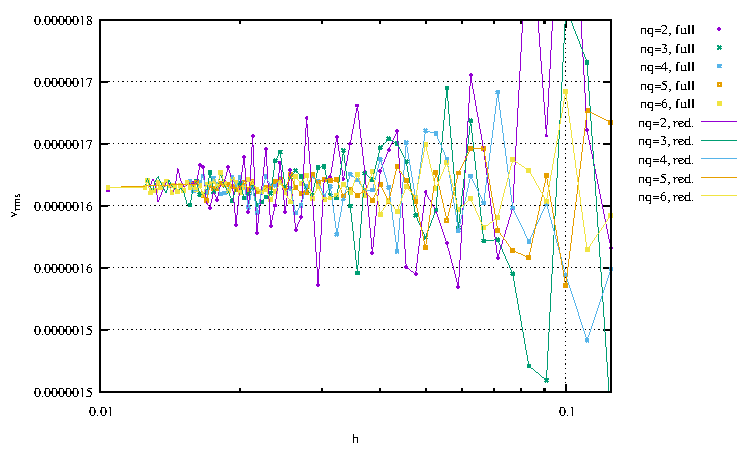
\includegraphics[width=9cm]{python_codes/fieldstone_80/results/sphere/vrms}\\
{\captionfont Root mean square velocity for $\delta \rho=0.001$, for both full density and reduced 
density models.}
\end{center}










